\subsection{Isolation Specifications}
\label{sec:ansi-isolation}

\begin{figure*}[t!]
\begin{smathpar}
\begin{array}{lcl}
(\A,\visZ) \Vdash \eta \in T_i & \defeq & \eta \in \A \conj \txn(\eta) = T_i\\
(\A,\visZ) \Vdash \eta_1 \visar \eta_2 & \defeq & \{\eta_1,\eta_2\}
        \subseteq \A \conj (\eta_1,\eta_2) \in \visZ\\
(\A,\visZ) \Vdash \eta_1 \soar \eta_2 & \defeq & \{\eta_1,\eta_2\}
        \subseteq \A \conj \txn(\eta_1)=\txn(\eta_2) \conj \id(\eta_1)
        < \id(\eta_2)\\
\E \Vdash S \subseteq T_i & \defeq & \forall \eta.~ \eta
        \in S \Rightarrow \underE{\eta \in T_i} \\
\E \Vdash T_i \visar \eta & \defeq &\forall\eta_1
        .\,(\E \Vdash \eta_1 \in T_i) \Rightarrow \E \Vdash \eta_1 \visar \eta \\
\underE{T_i \visar T_j} & \defeq &  \forall\eta_1,\eta_2.\,
    %\sameobj{\eta_1}{\eta_2}  \Rightarrow 
    \underE{\eta_1\in T_i} \conj \underE{\eta_2 \in T_j} \Rightarrow 
    \underE{\eta_1 \visar \eta_2} \\
\underE{T_i \invisar T_j} & \defeq &  \forall\eta_1,\eta_2.\,
        %\sameobj{\eta_1}{\eta_2}\Rightarrow 
        \underE{\eta_1\in T_i} \conj \underE{\eta_2 \in T_j} \Rightarrow 
        \neg (\underE{\eta_1 \visar \eta_2})\\
\underE{T_i \wrstoar X} & \defeq & \exists\eta.~
        \underE{\eta \in T_i} \conj \kind(\eta) = \C{WR}(X)\\
\underE{T_i \rdsfmar X} & \defeq & \exists\eta.~
        \underE{\eta \in T_i} \conj \kind(\eta) = \C{RD}(X)\\
\underE{T_i \usesar X} & \defeq & \underE{T_i \wrstoar X} \disj
      \underE{T_i \rdsfmar X}\\
\underE{\C{RMWVis}(T_j)} & \defeq & \forall\eta_1,\eta_2.\,
       \underE{\{\eta_1,\eta_2\} \subseteq T_j} \conj
       \underE{\eta_1 \soar \eta_2} \Rightarrow \underE{\eta_1 \visar
       \eta_2}\\
\underE{\C{MonotonicVis}(T_j)} & \defeq & 
       \underE{\C{RMWVis}(T_j)} \conj 
       \forall\eta,\eta_1,\eta_2.\, \underE{\{\eta_1,\eta_2\} \in T_j} 
          \conj \\
  &   & \hspace*{1.2in}\underE{\eta \visar \eta_1} \conj
        \underE{\eta_1 \soar \eta_2} \Rightarrow \underE{\eta \visar
        \eta_2} \\
%  \C{CausalVis}(T_i) & \defeq & 
%         \C{MonotonicVis}(T_i) \conj \C{RMWVis}(T_i)\\
\underE{\C{AtomicVis}(T_j)} & \defeq & 
       \forall\eta_1,\eta_2.\, \neg(\underE{\eta_1 \in T_j}) \conj
       \underE{\eta_2 \in T_j} \conj
       \underE{\eta_1 \visar \eta_2} \Rightarrow \underE{\txn(\eta_1)
       \visar \eta_2}\\
\underE{\C{CommitVis}(T_j)} & \defeq & 
       \forall\eta_1,\eta_2.~ \neg(\underE{\eta_1 \in T_j}) \conj 
          \underE{\eta_2 \in T_j} \conj
       \underE{\eta_1 \visar \eta_2} \Rightarrow\\
  &   & \hspace*{1.2in}\exists\eta.\, \underE{\eta \in \txn(\eta_1)} 
        \conj \kind(\eta) = \C{COMMIT} 
        \conj \underE{\eta \visar \eta_2}\\
% \underE{\C{TransVis}(T_j)} & \defeq &  \forall
%        \eta_1,\eta_2,\eta_3.\, \underE{\eta_3 \in T_j} \conj
%        \underE{\eta_1 \visar \eta_2} \conj
%        \underE{\eta_2 \visar \eta_3} \Rightarrow \underE{\eta_1 \visar
%        \eta_3} \\
\underE{\C{RC}(T_j)} & \defeq & \underE{\C{AtomicVis}(T_j)} 
        \conj \underE{\C{CommitVis}(T_j)}\\
\underE{\C{MAV}(T_j)} & \defeq & \underE{\C{RC}(T_j)} \conj
      \underE{\C{MonotonicVis}(T_j)} \\
\underE{\C{SnapshotVis}(T_i,T_j)} & \defeq &  \underE{T_i
       \visar T_j} \disj \underE{T_i \invisar T_j}\\
\underE{\C{RR}(T_j)} & \defeq & \underE{\C{MAV}(T_j)}
       \conj \forall T_i.\,T_i \neq T_j \Rightarrow 
        \underE{\C{SnapshotVis}(T_i,T_j)} \\
% &   & \hspace*{2in}\conj  \C{SnapshotVis}(T_i,T_j)\\
\underE{\C{SnapshotSER}(T_i,T_j,X)} & \defeq &  \underE{T_i
       \visar T_j} \disj (\underE{T_i \invisar T_j} \conj \\
  &   &\hspace*{1.2in}\exists \eta.~\underE{\eta\in T_i} \conj \kind(\eta) =
       \C{WR(X)} \Rightarrow \underE{T_j \visar \eta})\\
\underE{\C{SI}(T_j)} & \defeq &  \underE{\C{RR}(T_j)}
       \conj \forall T_i.\,(T_i \neq T_j \conj \exists X.\, \underE{T_i \wrstoar X} \conj 
        \underE{T_j \wrstoar X})\\
%      (\exists X.\, T_i \wrstoar X \conj T_j \wrstoar X)
%      \Rightarrow  \C{TotalVis}(T_i,T_j)\\
  &   & \hspace*{2in} \Rightarrow \underE{\C{SnapshotSER}(T_i,T_j,X)}\\
\underE{\C{SER}(T_j)} & \defeq & \underE{\C{RR}(T_j)}
        \conj \forall T_i.\,(T_i \neq T_j \conj \exists X.\, 
        \underE{T_i \wrstoar X} \conj \underE{T_j \usesar X})\\
  &   & \hspace*{2in} \Rightarrow \underE{\C{SnapshotSER}(T_i,T_j,X)}\\
\end{array}
\end{smathpar}

\caption{Standard isolation guarantees expressed as trace
well-formedness constraints}
\label{fig:ansi-isolation}
\end{figure*}

Fig.~\ref{fig:ansi-isolation} shows the specification of standard
isolation guarantees expressed as constraints over trace
well-formedness. For brevity and convenience, we adopt few notations
in this and subsequent sections.  An execution trace is destructed
into $\A$ and $\visZ$ whenever individual components of the pair are
needed. Otherwise, it is written as $\E$. Sometimes, the dot notation
(\eg~$\E.\A$) is also used. Since $\A$ and $\visZ$ are both sets, we
lift the operations on sets to pairs of sets when updating $\E$. For
example, $\E' = \E \cup (\{\eta_2\},\{(\eta_1,\eta_2)\})$ expands to
$\E' = (\E.\A \cup \{\eta_2\},\,\E.\visZ \cup \{(\eta_1,\eta_2)\})$.
When $\psi$ is a formula, $\underE{\psi}$ denotes the
interpretation of $\psi$ in the context of the trace $\E$. Such
interpretations are defined on a case-by-case basis in
Fig.~\ref{fig:ansi-isolation}. In the following, we give informal
explanations for each definition.

In the context of a trace $(\A,\visZ)$, an effect $\eta$ is said to
belong to a transaction $T_i$ if $\eta$ belongs to the effect set $A$
and its transaction identifier is $T_i$. The containment relation is
trivially lifted to the set of effects to define $\underE{S \subseteq
  T_i}$.  The interpretation of $\eta_1 \visar \eta_2$ and $\eta_1
\soar \eta_2$ are as explained earlier.  A transaction $T_i$ is said
to be visible to an effect $\eta$ if every effect $\eta_1$ of $T_i$
recorded by the trace is visible to $\eta$.  $T_i$ may be visible to
$\eta$ but may not be visible to every other effect in the
transaction. For a transaction $T_i$ to be considered to be visible to
a transaction $T_j$ in the context of a trace $\E$ (written
$\underE{T_i \visar T_j}$), every effect ($\eta_1$) of $T_i$ present
in $\E$ must be visible to every effect ($\eta_2$) of $T_j$ in
$\E$. Conversely, if none of the effects of $T_i$ present in $\E$ are
visible to any effect of $T_j$, then $T_i$ is considered invisible to
$T_j$ under $\E$ (written $\underE{T_i \invisar T_j}$). Transaction
$T_i$ is said to have written to a variable $X$ under $\E$ (i.e.,
$\underE{T_i \wrstoar X}$) if there exists a write-to-$X$ effect from
$T_i$ in $\E$. \emph{Reads-from} is similar. $T_i$ \emph{uses} $X$ if
it reads or writes $X$.

Various isolation guarantees are defined as propositions indexed by
a transaction identifier $T_j$. Transaction $T_j$ is said to have
experienced \emph{read-my-writes} visibility under $\E$ if every
effect ($\eta_1$) of $T_j$ is visible to every subsequent effect
($\eta_2$) of the same transaction in $\E$. This lets $T_j$ to never
lose its own updates. Monotonic visibility adds one more constraint to
read-my-writes; besides requiring $\eta_1$ to be visible to $\eta_2$,
it also requires every effect ($\eta$) visible to $\eta_1$ in $\E$ to
be visible to $\eta_2$ as well. Thus $T_j$ witnesses monotonically
increasing state as time progresses. Atomic visibility allows an
effect $\eta_2$ of $T_j$ to witness an effect $\eta_1$ of $T_i$ only
if all effects of $T_i$ in $\E$ are also visible to $\eta_2$. Atomic
visibility thus prevents a transaction from being partially visible.
However, atomic visiblity does not prevent an uncommitted
transaction from being visible. This is addressed by \C{CommitVis},
which requires the commit effect of $T_i$ to be visible whenever any
effect of $T_i$ is visible.

The ANSI SQL 92 standard requires \iso{Read Committted} isolation to avoid
the dirty reads phenomenon, which is achieved by enforcing
$\mathtt{AtomicVis}$ and $\mathtt{CommitVis}$ guarantees. The {\sc rc}
specification is therefore a combination of these two guarantees. The
specification also agrees with the description and
implementation~\cite{bailishat,pldi15} of {\sc rc} for highly
available replicated stores. On relational databases, however, {\sc
rc} has also come to be associated with the $\mathtt{MonotonicVis}$
guarantee.  Nonetheless, $\mathtt{AtomicVis}$ and $\mathtt{CommitVis}$
are sufficient to reason about {\sc rc} isolation on relational stores
too. The combination of these guarantees with the {\sc sc} property of
relational stores (formalized in \S\ref{sec:store-consistency})
automatically leads to the monotonicity guarantee, which explains why
{\sc rc} comes with $\mathtt{MonotonicVis}$ on such stores regardless
of the implementation. On weakly consistent stores however,
$\mathtt{AtomicVis}$ and $\mathtt{CommitVis}$ do not imply
$\mathtt{MonotonicVis}$. A stronger isolation level called
\iso{Monotonic Atomic View} ({\sc mav} of
Fig.~\ref{fig:ansi-isolation})~\cite{bailishat,pldi15} was proposed to
explicitly extend {\sc rc} with monotonicity on such stores. The sample
{\sc rc} executions shown in Fig.~\ref{fig:rc-executions} are also
{\sc mav}.

\begin{figure}
\centering
\subcaptionbox {
  {\sc rr}($T_1$), {\sc mav}($T_2$).
  \label{fig:ansi-iso-eg-rr}
} [
  0.33\columnwidth
] {
  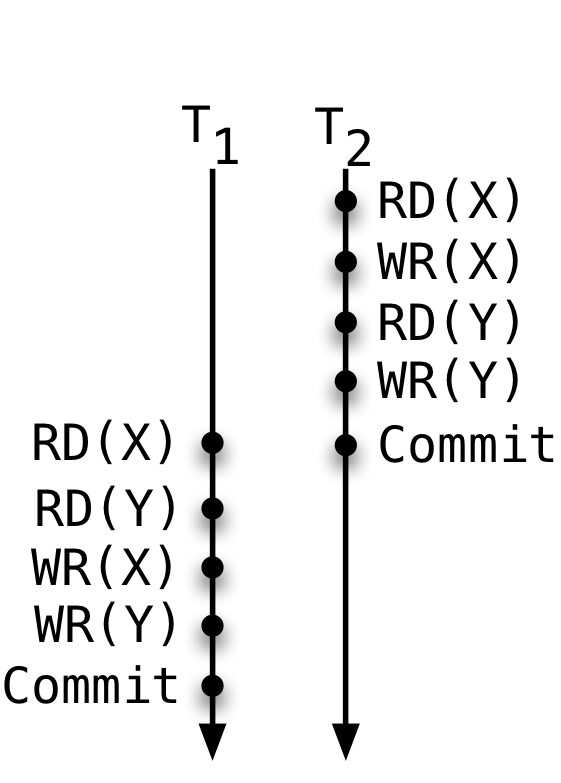
\includegraphics[scale=0.36]{Figures/rr-eg}
}
\subcaptionbox {
  {\sc si}($T_1$), {\sc mav}($T_2$)
  \label{fig:ansi-iso-eg-si}
} [
  0.33\columnwidth
] {
  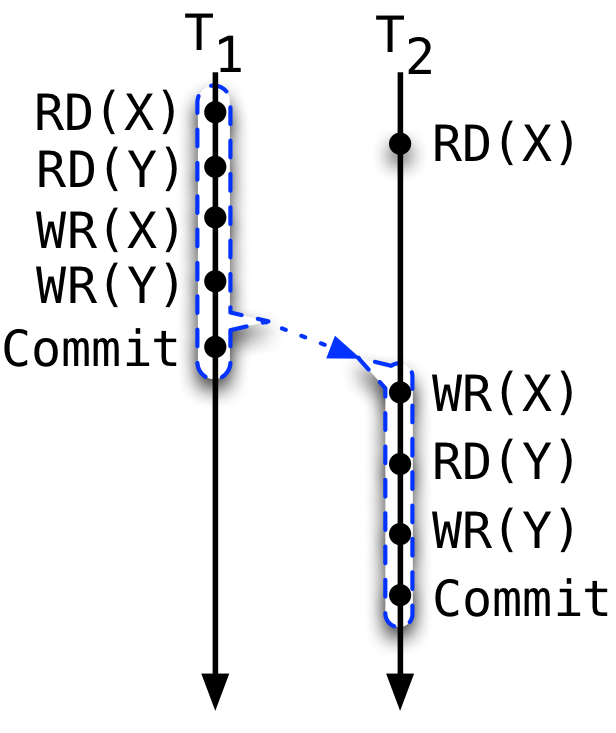
\includegraphics[scale=0.36]{Figures/si-eg-2}
}
\subcaptionbox {
  {\sc ser}($T_3$), {\sc mav}($T_4$)
  \label{fig:ansi-iso-eg-ser}
}{
  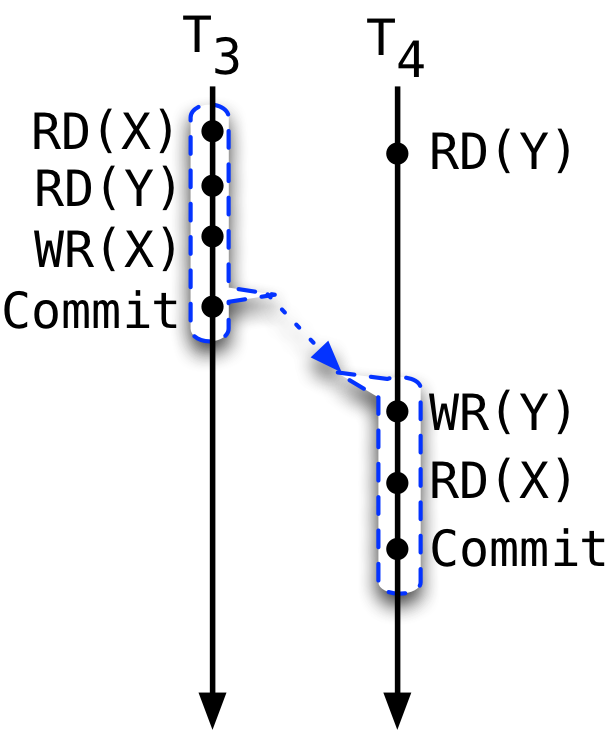
\includegraphics[scale=0.32]{Figures/ser-eg}
}

\caption{Sample executions of concurrent transactions at different
isolation levels. Solid (black) arrows indicate the timeline. Points
on the timeline mark the time when an operation is executed. Dotted
(blue) arrows denote $\visZ$. }
\label{fig:ansi-iso-eg}
\end{figure}

A transaction $T_i$ is said to be snapshot-visible to a transaction
$T_j$ if either it is visible to $T_j$, or it is invisible; it is
forbidden for only a suffix (more generally, a subset) of $T_j$ to
witness $T_i$.  \iso{Repeatable Read} ({\sc rr})
isolation extends {\sc mav} with the snapshot visibility guarantee.
Observe that snapshot visibility permits $T_i$ and $T_j$ to execute
and commit while being oblivious of each other. This scenario is
captured in Fig.~\ref{fig:ansi-iso-eg-rr}, where transactions $T_1$
and $T_2$, which perform conflicting writes, execute against a
snapshot of the database and commit concurrently. 

\iso{Snapshot Isolation} ({\sc SI}) proscribes this possibility. If
$T_i$ and $T_j$ both write to the same shared variable, then {\sc si}
insists that either $T_i$ be visible to $T_j$, or $T_j$ be visible to
the conflicting write of $T_i$ (this is captured by the auxiliary
definition \C{SnapshotSER}). Fig.~\ref{fig:ansi-iso-eg-si} shows an
execution where {\sc si} transaction $T_1$ witnesses a snapshot of the
database that doesn't include $T_2$, but the conflicting write to $X$
in $T_2$, and the subsequent operations (due to the monotonicity
requirement of {\sc mav}) witness $T_1$. Thus, $T_2$ is aware of $T_1$
when it commits. Lastly, \iso{Serializable} isolation extends
$\mathtt{SnapshotSER}$ to also cover non-conflicting transactions that
write to variables read in the current transaction.
Fig.~\ref{fig:ansi-iso-eg-ser} shows an execution of an {\sc ser}
transacton $T_3$ and a {\sc mav transaction} $T_4$, which write to $X$
and $Y$, respectively. The snapshot witnessed by the {\sc ser}
transaction $T_3$ does not include $T_4$, but the write to $Y$ in
$T_4$, although non-conflicting, witnesses $T_1$ because $Y$ is read
by $T_1$. Visibility includes other operations of $T_4$ because of
{\sc mav}.

% Note that both $\mathtt{SnapshotVis}$ and $\mathtt{OneWaySER}$
% are asymmetric definitions that guarantee complete visiblity or
% invisibility of $T_i$ to $T_j$, but not the converse. While
% $\mathtt{SnapshotVis}$ provides no guarantees to $T_i$,
% $\mathtt{OneWaySER}$ guarantees that at least the commit effect of
% $T_i$ witnesses $T_j$. 

% \iso{Snapshot Isolation} spec ({\sc si}) extends {\sc rr} with a
% one-way serializability guarantee w.r.t the transactions that perform
% conflicting writes (i.e., writes to the same shared variable).
% \footnote{Fig.~\ref{fig:ansi-isolation} presents slightly
% weaker versions of {\sc si} and {\sc ser} specs in the interest of
% clarity.}. Fig.~\ref{fig:ansi-iso-eg} shows sample executions of
% transactions $T_1$ and $T_2$. Both transactions read and write to
% shared variables $X$ and $Y$. In the first execution, $T_2$ commits
% while $T_1$ is still in progress, but {\sc rr} isolation prevents
% $T_1$ from witnessing the writes of $T_2$. In the second execution,

%% SJ: Not sure this paragraph is necessary here.
%% In contrast to recent proposals (\emph{e.g.},
%% ~\cite{gotsmanconcur15}), our specifications for {\sc si} and {\sc
%%   ser} do not necessarily impose a total order among transactions
%% (conflicting or otherwise). In reality, a total order under {\sc ser}
%% (resp. {\sc si}) is guaranteed only if the store executes all
%% transactions under {\sc ser} (resp. {\sc si}) isolation. Our
%% specifications admit this possibility, and derive a total order under
%% the assumption of homogenity. However, databases almost always allow
%% isolation levels to be configured on a per-transaction basis, allowing
%% transactions at various isolation levels to coexist.  Specifications
%% that assume homogenity are incorrect under this setting.

% Having specified isolation levels as trace well-formedness
% constraints, we can now construct trace invariants ($\I$) for
% \txnimp programs by composing isolation specifications for various
% transactions. For instance, the following trace invariant enforces
% {\sc si} for both transactions of the program in
% Fig.~\ref{fig:motiv-eg-1}, allowing it to satisfy its postcondition:
% \begin{smathpar}
% \I \;=\; \lambda\E.~ \underE{\C{SI(Wd1)}} \conj \underE{\C{SI(Wd2)}}
% \end{smathpar}
% In contrast, the following trace invariant enforces {\sc rc} for one and {\sc si}
% for another, leading to a possible violation of the postcondition:
% \begin{smathpar}
% \I \;=\; \lambda\E.~ \underE{\C{RC(Wd1)}} \conj \underE{\C{SI(Wd2)}}
% \end{smathpar}
